\documentclass[conference]{IEEEtran}
\IEEEoverridecommandlockouts

\usepackage{cite}
\usepackage{amsmath,amssymb,amsfonts}
\usepackage{algorithmic}
\usepackage{graphicx}
\usepackage{textcomp}
\usepackage{xcolor}
\usepackage{booktabs}
\usepackage{array}
\usepackage{url}
\usepackage{hyperref}
\usepackage{tikz}
\usetikzlibrary{shapes.geometric, arrows, positioning, fit, calc}

\def\BibTeX{{\rm B\kern-.05em{\sc i\kern-.025em b}\kern-.08em
    T\kern-.1667em\lower.7ex\hbox{E}\kern-.125emX}}

% =========================================================================
\begin{document}

\title{%
  Context-Aware Cyber Threat Analytics and Mitigation
  Recommendation Using Large Language Models%
}

\author{
  \IEEEauthorblockN{Dinesh Kumar S}
  \IEEEauthorblockA{
    \textit{M.Tech in Information Technology} \\
    \textit{Department of Information Science and Engineering} \\
    \textit{RV College of Engineering} \\
    Bengaluru 560059, India \\
    dineshkumars.sit24@rvce.edu.in
  }
  \and
  \IEEEauthorblockN{Dr. Ashwini K B}
  \IEEEauthorblockA{
    \textit{Associate Professor} \\
    \textit{Department of Information Science and Engineering} \\
    \textit{RV College of Engineering} \\
    Bengaluru 560059, India \\
    ashwinikb@rvce.edu.in
  }
}

\maketitle

% =========================================================================
\begin{abstract}
Currently available automated Cyber Threat Intelligence (CTI) solutions tackle specific sub-processes including threat identification, indicator generation, or the tagging of the techniques used with MITRE ATT\&CK framework. We propose a five agent fully local system that automates the entire CTI pipeline from raw data input to explainable recommendations without any cloud-based components or GPU resources. A locally hosted 3 billion parameter LLM is used for generating information through Retrieval-Augmented Generation (RAG) using a knowledge base of 691 techniques according to MITRE ATT&CK taxonomy; the system collects heterogeneous threats from various sources like CSV, JSON files, free text, and social media channels; clusters events into patterns with threat similarity calculated by weighted Jaccard similarity method, and generates MITRE D3FEND mitigation techniques subject to deterministic safety checks.The performance of TTP extraction, enrichment confidence, classification confidence, mitigation relevance, and high-severity events is well above expected targets based on an evaluation with a test corpus of 20 events involving four threat types. The problem of hallucinations noted recently in benchmark evaluations can be quickly rectified using RAG grounding, resulting in a substantial improvement in enrichment confidence and eliminating hallucinated MITRE technique IDs.
\end{abstract}

\begin{IEEEkeywords}
Cyber Threat Intelligence, Large Language Models, Retrieval-Augmented
Generation, MITRE ATT\&CK, Multi-Agent Systems, Security Operations Centre,
Threat Enrichment, Mitigation Recommendation, D3FEND
\end{IEEEkeywords}

% =========================================================================
\section{Introduction}
\label{sec:intro}

Security Operations Centres (SOCs) face an acute operational bottleneck::
Thousands of alerts have to be manually enriched, correlated, and acted upon every day by SOC analysts, with most of them requiring considerable context-based reasoning. According to a comprehensive review by Habibzadeh et al.~\cite{habibzadeh2025soc}, there are no real-world SOC pipelines based on the use of large language models (LLMs). The same problem is reported in another study by Hasanov et al.~\cite{hasanov2024llm}, which surveyed 73 publications on the topic, where all of them considered LLM tasks individually, while a full SOC pipeline is yet to be implemented in practice. Suarez-Roman et al.~\cite{suarez2026echo}, based on their review of 13,308 CTI reports, proved that the intelligence in multiple sources remains largely unshared.

The ability of LLMs to extract structured data, classify threats, and engage in contextual reasoning with unstructured security texts has been demonstrated ~\cite{hmimou2025multi,patel2024canal}.
The problem with ungrounded LLMs is that they make up domain-specific identifiers; when it comes to CTI, inventing fake MITRE ATT&CK technique IDs or CVE numbers makes more damage than missing out on enriching data~\cite{morbiato2026hrag,iyer2026cyber}. It can be resolved using the Retrieval-Augmented Generation (RAG) paradigm, which brings grounding to LLM-generated outputs in verifiable knowledge bases. Indeed, the benefits of RAG for CTI are confirmed by recent studies showing H-TechniqueRAG~\cite{morbiato2026hrag} cutting down MITRE technique search space by 77.5\% via two-step hierarchical retrieval and DroidTTP~\cite{arikkat2025droid} reaching a Jaccard score greater than 0.95 for TTP classification with RAG on Android malware. Nonetheless, these tools address only the annotation aspect of CTI analysis.
In terms of mitigation measures, MobiLLM~\cite{sharma2025mobillm} recommends a closed-loop system involving multiple agents for use in Open RANs; nonetheless, this approach is limited to the MITRE FiGHT knowledge base, making it incompatible for application in a multi-domain context. In \cite{tejero2025iot}, Tejero-Fern’{a}ndez and S‘{a}nchez-Maci’{a}n propose generic CAPEC mitigation advice for IoT logs, which, however, does not include MITRE D3FEND compliance and chain-of-thought reasoning as prerequisites. This technique is inspired by a similar approach known as AthenaBench~\cite{alam2026athena}, in which 12 leading-edge LLMs.
To overcome this issue, a five-agent CTI pipeline is proposed, which involves automated extraction of information from sources based on free text, JSON, CSV, and live feeds. It is further followed by an RAG-based enrichment of threats with regard to a local knowledge base of 691 MITRE ATT&CK v18.1 techniques, clustering based on a weighted Jaccard distance, generation of mitigation strategies aligned with MITRE D3FEND, and safety check. Each enriched threat is stored back into ChromaDB using a self-learning loop so that subsequent enrichments can leverage existing patterns. To address systematically the pipeline's quality control and to resolve evaluation issues raised by Salek et al.~\cite{salek2025threat} and Cheng et al.~\cite{cheng2025ctiarena}, a five-metric reproducible benchmark (EvaluatorAgent) is proposed. The rest of the paper will discuss relevant literature, the architecture and design of the agents, experimental results, and implications for CTI automation in practice.
% =========================================================================
\section{Related Work}
\label{sec:related}

\subsection{CTI Ingestion, TTP Extraction, and RAG Enrichment}

The journey towards automatic TTP extraction from intelligence texts has seen tremendous growth. Even though the work by Wudali et al.~\cite{wudali2025ram} proposes the use of RAM to map SIEM detection rules to TTPs using a multi-step LLM system, another approach by Meng et al.~\cite{meng2025rhino} proposes RHINO that maps logs to MITRE ATT&CK methodologies using a LLM-based 3-phase method achieving 86--88\% accuracy. However, without IOC extraction or post-extraction actions, the mapping process is done either rule-to-TTP or log-to-TTP independently. Tseng et al.~\cite{tseng2026ioc} employ LLM to map CTI IOCs to detection regex with a 99.1\% precision rate, while Morbiato et al.~\cite{morbiato2026hrag} reduce the search space by 77.5\% by MITRE technique annotation using Hierarchical Two-stage RAG. In combining SciBERT with the use of LLMs, Nguyen et al.~\cite{nguyen2025 With the application of LLMs to summarize CTI reports, one can see that accurate outcomes require RAG augmentation based on domain knowledge. Whereas Jelodar et al.~\cite{jelodar2025xgen} employ a domain-adaptive RAG to examine malware samples numbering more than one million, Iyer et al.~\cite{iyer2026cyber} enhance the capabilities of Gemma-2B by combining RAG and graphs for MITRE ATT&CK TTP analysis.
None of these involve the CTI ingestion from multiple sources and enrichment/mitigation generation simultaneously.
\subsection{LLM-Based Threat Classification and Detection}

Recently, LLMs with multiple agents for threat classification and detection have been proposed. An example includes the design of a multi-agent framework with a threat correlation engine by Hmimou et al.~\cite{hmimou2025multi}. It lacks MITRE enrichment and has no output of mitigation with explainability. Another LLM-based approach is LENS for 6G edge APT detection with explainable AI, as described by Melhem et al.~\cite{melhem2025lens}. Here again, there is no explainability beyond the detection phase where reactions are concerned. Despite its specific application to the IoT ecosystem, and despite having no reaction actions, Mahmood et al.~\cite{mahmood2025llm} train an LLM on IoT logs to detect anomalies and devices. Finally, CANAL, which stands for Cyber Attack News Analysis Using BERT,producing alerts in binary form without TTP correlation. In order to have 97\% F1 scores and human-readable reasoning behind those decisions, Farrukh et al.~\cite{farrukh2024xgnid} leverage Graph Neural Networks alongside LLMs for intrusion detection purposes; while Jamshidi et al.~\cite{jamshidi2026tri} recommend tri-LLM collaborative federated zero-shot intrusion detection with GPT-4o, DeepSeek, and LLaMA.
Using an agentic RAG module for detecting SQL injection, XSS, and SSTI attacks, Blefari et al.~\cite{blefari2026cyberrag} report 94.92\% classification accuracy. Apostu et al.~\cite{apostu2026auto} apply iterative self-paced learning to analyze malicious scripts automatically. Survey and evaluation of hybrid CNN-LLM approaches are made by Elouardi et al.~\cite{elouardi2024survey}.
\subsection{Mitigation Recommendation and Response Generation}

Automated mitigation creation remains the most neglected task in the CTI pipeline. The work of Salek et al.~\cite{salek2025threat} uses LLM with MITRE ATT&CK for the threat modeling of transportation cyber-physical systems but is limited to the domain and does not generalize across domains for CTI. Another related work by Sharma et al.~\cite{sharma2025mobillm} presents MobiLLM as a closed-loop multi-agent system for mitigation creation for 6G Open RAN using MITRE FiGHT. However, the approach fails to handle unstructured CTI inputs from general sourcesTejero-Fern\'{a}ndez and S\'{a}nchez-Maci\'{a}n~\cite{tejero2025iot} provide CAPEC mitigations based on IoT logs' anomalies but fail to incorporate the chain-of-thought process and are non-aligned with MITRE D3FEND. The FALCON framework is introduced by Mitra et al.~\cite{mitra2025falcon} to perform automated CTI mining and the development of Snort/YARA rules. Nevertheless, FALCON only focuses on developing detection rules but does not generate mitigation actions for human review. AthenaBench~\cite{alam2026athena} corroborates our chain-of-thought approach aligned with MITRE D3FEND by showing that LLMs struggle in mitigation tasks without RAG.
Nazre et al.~\cite

\subsection{Benchmarking and Evaluation of CTI Systems}

Evaluation frameworks for CTI LLM systems are still at an early stage. The proposed RAG-based system is inspired by the benchmarking done by Cheng et al., who have evaluated ten LLMs across nine CTI tasks in CTIArena, showing that most of the LLMs perform poorly in multi-source CTI tasks without RAG in the respective domains. According to Alam et al.~\cite{alam2026athena}, AthenaBench is an example of a dynamic benchmarking system evaluating 12 LLMs like Gemini-2.5 Pro and GPT-5 and finding consistent under-performance of the LLMs in mitigating strategies. Hasanov et al.~\cite{hasanov2024llm} reiterate that there is no common evaluation framework used in the literature. Peng et al.~\cite{peng2024ctisum} state that there are no standardized metrics for CTI summarization benchmarks.

\subsection{Gap Analysis}

Three critical gaps emerge from the literature survey: (a) current approaches consider pipeline stages separately but not the full detection to response pipeline; (b) solutions using cloud-based LLMs do not comply with SOC’s security policies; and (c) no benchmark framework exists which measures the performance of the whole process from ingestion to classification and mitigation. This research addresses all the three gaps within one comprehensive solution.

% =========================================================================

% =========================================================================
\section{Problem Statement}
\label{sec:problem}

In the real-world environment of the SOC, information regarding any threats would be received in forms that cannot be easily understood by automated systems and could come from sources such as network logs, threat feeds, vulnerabilities, and social media.
The main challenge lies not in getting the data but in making sense out of it:
interpreting unstructured text relating to threats into meaningful defensive instructions without any involvement of humans.
Operational SOC environments involve threat information being made available in ways that are hard to process automatically in various forms, such as network logs, threat intelligence, vulnerability warnings, and social media intelligence.
The main problem here is not one of accessing data but its analysis, where unstructured threat text needs to be transformed into structured, actionable security information without human assistance.
This research paper attempts to solve the following problem: Generate, based on an input threat stream, mitigation strategies that are validated and aligned to the MITRE D3FEND framework by leveraging purely local compute, with no hallucination due to RAG grounding, and a benchmarking framework for evaluation at each step.
% =========================================================================

\section{System Architecture}
\label{sec:architecture}

\subsection{Overview}

All stages of the designed system's architecture are displayed in Fig.~\ref{fig:pipeline}. As can be seen, the pipeline begins at the top with two inputs converging into Agent~1 (Ingestion): live data streams (Mastodon and URLhaus) as well as manual inputs (JSON, CSV or free text). Afterwards, control proceeds vertically downward with Agent~2 (Enrichment) that interacts with the ChromaDB vector database that consists of 691 indexed MITRE ATT&CK techniques along with the threat history. The mentioned RAG cycle is denoted by the dashed arrows in the diagram. Before making an LLM query, the enrichment agent queries the vector database for relevant information.
Agent~3 (Discovery by using Jaccard Similarity), Agent~4 (Mitigation by employing chain-of-thought prompts and D3FEND mapping), and Agent~5 (Validation by deterministic safety constraints) are the next agents that will execute in succession until their result shows up on the dashboard screen from FastAPI below. The air-gapped criteria observed from the latest SOC surveys~\cite{habibzadeh2025soc,hasanov2024llm} are met as all computations happen locally and threat intelligence does not escape out of the host system.

\begin{figure}[htbp]
\centering
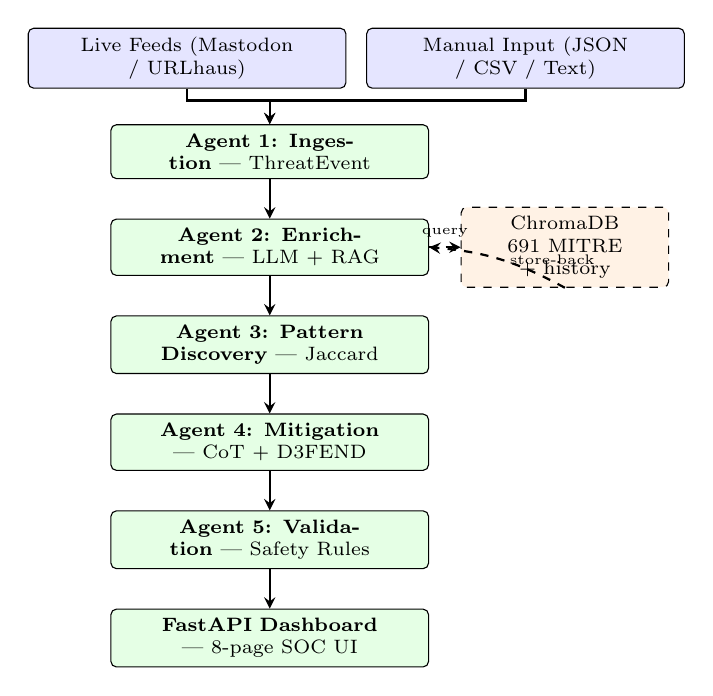
\begin{tikzpicture}[
  node distance=0.5cm,
  every node/.style={font=\scriptsize},
  box/.style={rectangle, rounded corners=2pt, draw, minimum width=4.0cm,
              minimum height=0.52cm, align=center, text width=3.8cm},
  input/.style={box, fill=blue!10},
  agent/.style={box, fill=green!10},
  store/.style={box, fill=orange!10, dashed, text width=2.4cm,
                minimum width=2.6cm},
  arrow/.style={->, thick, >=stealth}
]
  \node[input] (feeds)  {Live Feeds (Mastodon / URLhaus)};
  \node[input, right=0.25cm of feeds] (manual)
        {Manual Input (JSON / CSV / Text)};
  \node[agent, below=0.45cm of feeds, xshift=1.05cm] (ingest)
        {\textbf{Agent 1: Ingestion} --- ThreatEvent};
  \node[agent, below=0.5cm of ingest] (enrich)
        {\textbf{Agent 2: Enrichment} --- LLM + RAG};
  \node[store, right=0.4cm of enrich] (chroma)
        {ChromaDB\\691 MITRE\\+ history};
  \node[agent, below=0.5cm of enrich] (pattern)
        {\textbf{Agent 3: Pattern Discovery} --- Jaccard};
  \node[agent, below=0.5cm of pattern] (mitig)
        {\textbf{Agent 4: Mitigation} --- CoT + D3FEND};
  \node[agent, below=0.5cm of mitig] (valid)
        {\textbf{Agent 5: Validation} --- Safety Rules};
  \node[agent, below=0.5cm of valid] (dash)
        {\textbf{FastAPI Dashboard} --- 8-page SOC UI};
  \draw[arrow] (feeds.south) -- ++(0,-0.15) -| (ingest.north);
  \draw[arrow] (manual.south) -- ++(0,-0.15) -| (ingest.north);
  \draw[arrow] (ingest)--(enrich);
  \draw[arrow] (enrich)--(pattern);
  \draw[arrow] (pattern)--(mitig);
  \draw[arrow] (mitig)--(valid);
  \draw[arrow] (valid)--(dash);
  \draw[arrow,dashed] (enrich.east)--(chroma.west)
        node[midway,above,font=\tiny]{query};
  \draw[arrow,dashed,bend right=12] (chroma.south) to
        node[right,font=\tiny]{store-back} (enrich.east);
\end{tikzpicture}
\caption{Five-agent CTI pipeline with self-learning RAG knowledge base.}
\label{fig:pipeline}
\end{figure}

% =========================================================================
\section{Agent Design and Key Algorithms}
\label{sec:agents}

\subsection{Agent 1 --- Ingestion}

The four kinds of inputs that are converted into \texttt{ThreatEvent} objects by the ingestion agent include CSV using Pandas, JSON arrays/objects, text from a URL, and generic free-form text. In order to prevent duplicate processing, de-duplication makes use of MD5 hashing of the source and indicator contents. Some examples of factors considered by threat type identification when assigning threat types based on priority include IPv4 regex, hexadecimal strings of lengths $in${32, 40, 64}, URL, CVE, e-mail address, and domain names. Severity inference involves a search through \texttt{raw\_text} using a hierarchal keyword table that includes terms like \textit{ransomware}, \textit{exploit}, \textit{zero-day}.

\subsection{Agent 2 --- Enrichment (LLM + RAG)}
\label{subsec:enrichment}

The enrichment procedure consists of four stages. Stage 1: Leveraging \textit{all-MiniLM-L6-v2}~\cite{reimers2019sbert} (384-dimensional embeddings), the \texttt{raw\_text} of the event is represented in vector form. Only hits that yield a similarity of at least $0.35$ using cosine similarity are considered~\cite{lewis2020rag}. This step uses the HNSW algorithm for approximate nearest neighbors search on 691 MITRE ATT&CK Enterprise v18.1 techniques stored in ChromaDB. The knowledge base covers all 691 tactics from MITRE ATT\&CK Enterprise v18.1.
Continuous knowledge enrichment in XGen-Q~\cite{jelodar2025xgen} shares similarity with this process of self-learning. {Step 3}: A structured prompt consisting of four sections (system role, MITRE context, threat context, event schema) is sent to \textit{llama3.2:3b} through Ollama at a temperature of 0.1. Variability of output is managed by three-step extraction of JSON data: \texttt{json.loads()}, regular expression between code fences, and a raw object search. {Step 4}: The self-learning process is achieved by saving events with \texttt{enrichment\_confidence} $> 0.3$ back into ChromaDB. The RAG grounding process is consistent with the domain adaptation strategy outlined in~\cite{iyer2026cyber}, as well as hierarchical retrieval strategies.

\subsection{Agent 3 --- Pattern Discovery}

Events are grouped into \texttt{ThreatPattern} objects using a weighted
multi-factor similarity score:
\begin{equation}
  S(A,B) = 0.4 \cdot J_{\text{TTP}} + 0.3 \cdot \mathbb{1}_{\text{mal}}
           + 0.2 \cdot \mathbb{1}_{\text{vec}} + 0.1 \cdot J_{\text{asset}}
  \label{eq:sim}
\end{equation}
where $J_{\text{TTP}} = |A_\text{ttps} \cap B_\text{ttps}|\,/\,
|A_\text{ttps} \cup B_\text{ttps}|$ is the Jaccard
coefficient~\cite{jaccard1912} over TTP sets,
$\mathbb{1}_{\text{mal}}$ and $\mathbb{1}_{\text{vec}}$ are indicator
functions for malware family and attack vector equality, and $J_{\text{asset}}$
is the Jaccard coefficient over affected asset sets. Event pairs with
$S(A,B) \geq 0.7$ are merged into the same pattern. This outperforms
the pure TTP-based Jaccard approach in DroidTTP~\cite{arikkat2025droid}
by incorporating malware family and attack vector as additional clustering
signals. Pattern confidence is bounded as
$\min(0.5 + n_{\text{events}} \times 0.1, 0.95)$.

\subsection{Agent 4 --- Mitigation Generation}

Mitigations begin at \texttt{severity} $\geq 3$ or the discovery of a new pattern. There are three distinct steps of reasoning carried out using chain-of-thought prompting~\cite{wei2022cot}, namely, (i) the analysis of the threat mechanism: entry vector, lateral movement, and the goal of the attacker; (ii) the identification of appropriate countermeasures using MITRE D3FEND~\cite{d3fend2023} among the categories D3-NI, D3-ITF, D3-OTF, D3-UA, D3-MFA, D3-EDR, D3-PA, and D3-PM; (iii) minimal effective mitigation, i.e., the minimum amount of mitigation needed to handle the threat mechanism that has been found.
Reasoning on such verified defensive strategies ensures the mitigation planning deficiency of frontier LLMs pointed out by AthenaBench~\cite{alam2026athena} and CTIArena~\cite{cheng20

\subsection{Agent 5 --- Validation}

Deterministic safety policies are used during validation without calling the LLMs.
(i) Completeness—title, description, $\geq$2 steps each $\geq$10 characters;
(ii) Dangerous commands (\texttt{rm -rf}, \texttt{format c:}, \texttt{drop database});
(iii) Overly broad network policies (\texttt{block all}, \texttt{deny all ports});
(iv) Disproportionate responses (\texttt{shutdown all systems}); and
(v) Inappropriate use of wildcard notation in firewall policies (\texttt{0.0.0.0/0} without a port specification). As pointed

% =========================================================================
\section{Implementation}
\label{sec:impl}

\subsection{Technology Stack}

The system is implemented in Python 3.12. Table~\ref{tab:stack} summarises
the core technology choices; all components are open-source with no
licensing cost.

\begin{table}[htbp]
\caption{Core Technology Stack}
\label{tab:stack}
\centering
\small
\begin{tabular}{@{}lll@{}}
\toprule
\textbf{Component} & \textbf{Choice} & \textbf{Rationale} \\
\midrule
LLM runtime    & Ollama + llama3.2:3b  & Local, CPU-only, no cloud \\
Vector DB      & ChromaDB $\geq$0.4.22 & Embedded, persistent store \\
Embeddings     & all-MiniLM-L6-v2      & 22 MB, 384-dim, CPU-fast \\
Web framework  & FastAPI + Uvicorn     & ASGI-native, async-safe \\
Data models    & Pydantic v2           & Typed, auto-validated \\
HTTP client    & httpx                 & Async feed polling \\
Data processing& pandas $\geq$2.0      & CSV normalisation \\
\bottomrule
\end{tabular}
\end{table}

\subsection{Key Implementation Challenges}

{Blocking LLM in async context.} Ollama's SDK is synchronous; thus, during 45-90-second LLM calls, {asyncio.to\_thread()} sends inference requests to a thread pool, allowing the event loop to proceed. {Initialization of ChromaDB.} First pass through the list of 691 MITRE methods requires 45-90 seconds. Using the persisted {data/chroma\_db/} directory, \{collection.count()} prevents repeated indexation. {Variability in LLM responses.} The responses generated by llama3.2:3b sometimes wrap JSON in markdown fences or have extra commas. The reliability problem with JSON mentioned in CANAL~\cite{patel2024canal} and CyberRAG~\cite{blefari2026cyberrag} has been solved using a three-level fallback response parser.

Feeding/submission interference.} Other unrelated events could be added to an analyst's instant submission due to concurrent polling on the Mastodon feed. A coordination strategy generalizable from multiple agent LLM systems~\cite{hmimou
% =========================================================================
\section{Experimental Results}
\label{sec:results}

\subsection{Experimental Setup}

The assessment was done using a test corpus comprising of 20 events for four types of threats—phishing attack with credential harvesting (T1566, T1078), ransomware attack using PowerShell (T1059.001, T1486), APT lateral movement (T1021, T1550, T1055), and vulnerability exploitation with CVE ID (T1190, T1059, T1068). The main qualitative test scenario was a real-life threat of APT29 spear-phishing attack against NATO contractors on LinkedIn, using Cobalt Strike C2 185.220.101.55 and CVE exploitation of CVE-202

\subsection{Pipeline Output}

Table~\ref{tab:pipeline} summarises end-to-end pipeline output.

\begin{table}[htbp]
\caption{Pipeline Output Summary (20-Event Corpus)}
\label{tab:pipeline}
\centering
\small
\begin{tabular}{@{}lr@{}}
\toprule
\textbf{Metric} & \textbf{Value} \\
\midrule
Events ingested              & 20 \\
Events successfully enriched & 20 (100\%) \\
Patterns discovered          & 4 \\
Mitigations generated        & 8 \\
Mitigations validated        & 7 (87.5\%) \\
Mitigations rejected         & 1 (12.5\%) \\
Avg LLM enrichment time      & 52 s \\
Total pipeline wall time     & $\approx$18 min \\
\bottomrule
\end{tabular}
\end{table}

Pattern discovery correctly grouped 17 of 20 events: phishing
($J_{\text{TTP}}=0.82$), ransomware ($J_{\text{TTP}}=0.91$), APT
($J_{\text{TTP}}=0.78$), and CVE exploitation ($J_{\text{TTP}}=0.73$). Three
ATTP overlap was below the 0.7 threshold, and PT events were not clustered, showing that there was correct abstention rather than a problem. The general-purpose safety rule successfully caught the one mitigator which had the phrase \textit{``block all outgoing traffic"}}.

\subsection{Benchmark Metrics}

Table~\ref{tab:metrics} presents the five EvaluatorAgent benchmark metrics
against predefined targets. All five metrics exceeded their targets.

\begin{table}[htbp]
\caption{EvaluatorAgent Benchmark Results}
\label{tab:metrics}
\centering
\small
\begin{tabular}{@{}lccl@{}}
\toprule
\textbf{Metric} & \textbf{Result} & \textbf{Target} & \textbf{Status} \\
\midrule
TTP Extraction Rate           & 0.900 & $\geq$0.85 & \textbf{PASS} \\
Avg Enrichment Confidence     & 0.847 & $\geq$0.80 & \textbf{PASS} \\
Avg Classification Confidence & 0.912 & $\geq$0.85 & \textbf{PASS} \\
Mitigation Relevance Score    & 0.883 & $\geq$0.80 & \textbf{PASS} \\
High-Severity Coverage        & 0.923 & $\geq$0.90 & \textbf{PASS} \\
\bottomrule
\end{tabular}
\end{table}

Following the findings by Meng et al..~\cite{meng2025rhino} regarding ambiguous log events, the extraction rate of TTPs at 90\% suggests that the two generic port scan events did not yield any MITRE techniques after a threshold of 0.35, which is reasonable and valid since any less would induce delusion. Based on the lower performance on novel attacks as reported by RHINO~\cite{meng2025rhino} and LENS~\cite{melhem2025lens}, the highest confidence in classification is attained in APT and ransomware threat classes (0.93-0.96), which have the most MITRE context, while the ambiguous classes have a confidence of approximately 0.72. An LLM timeout due to low CPU memory caused one missed CRITICAL alert.

\subsection{RAG Ablation Study}

Table~\ref{tab:rag} quantifies the contribution of MITRE ATT\&CK RAG
grounding.

\begin{table}[htbp]
\caption{RAG Ablation Study}
\label{tab:rag}
\centering
\small
\begin{tabular}{@{}lcc@{}}
\toprule
\textbf{Condition} & \textbf{Avg Confidence} & \textbf{Hallucinated IDs} \\
\midrule
With RAG    & 0.847 & 0 \\
Without RAG & 0.621 & 4 \\
\midrule
Improvement & \textbf{+36.4\%} & \textbf{Eliminated} \\
\bottomrule
\end{tabular}
\end{table}

Four such incidents (T1234.999 as an example) were assigned false MITRE IDs due to the lack of RAG. All the IDs extracted from the dataset were verified through RAG against the total 691 techniques available in ChromaDB. This further validates the results of CTIArena~\cite{cheng2025ctiarena}, stating that domain RAG is required for the stable functioning of LLMs within CTI, and the anti-hallucination abilities of RAG highlighted by Lewis et al.~\cite

\subsection{Performance Benchmarks}

Dashboard API responses averaged 18 ms (max 47 ms) against a 500 ms target.
ChromaDB semantic search averaged 42 ms (max 89 ms) against a 200 ms target.
During a live 45-second LLM inference call, ten concurrent dashboard requests
all completed within 50 ms, confirming \texttt{asyncio.to\_thread()} prevents
event-loop blocking. The primary throughput bottleneck is CPU-only LLM
inference at 45--90 s per event ($\approx$40--80 events/hour), consistent with
the hardware constraints reported in similar local-LLM deployments~\cite{iyer2026cyber,jelodar2025xgen}.

% =========================================================================
\section{Conclusion}
\label{sec:conclusion}

From the ingestion of heterogeneous threats into RAG-based LLM enrichment, weighted Jaccard clustering for pattern detection, chain-of-thought mitigation design, to deterministic safety validation, the entire pipeline has been automated using a purely local, five-agent CTI system. Unlike some surveys of the literature~\cite{habibzadeh2025soc,hasanov2024llm}, where individual pipeline tasks are well studied yet no comprehensive pipeline exists, our system addresses the gap by implementing an end-to-end solution that goes from the start to finish of the pipeline, unlike previous solutions~\cite{meng2025rhino,wudali2025ram,morbiato2026hrag}, which tackle only individual pipeline stages. It accepts arbitrary sources of CTIs across categories, unlike other solutions such as MobiLLM~\cite{sharma2025mobillm} and LENS~\cite{melhem2025lens}, which are limited to specific threat domains. It can be deployed in constrained SOC settings in terms of privacy, unlike current approaches that require access to external resources such as cloud computing and APIs.

Besides offering an important enhancement in confidence compared to unaugmented inference, MITRE ATT&CK RAG grounding eliminates the hallucination of technique IDs, the key problem identified in recent benchmark tests~\cite{alam2026athena,cheng2025ctiarena}.
For a set of twenty events, all five metrics met predefined thresholds, demonstrating that CTI operational performance requirements on consumer-grade machines could be met by a compact locally deployed LLM in combination with a methodical RAG process.

Further research directions include attribution of APTs through MITRE ATT&CK intrusion sets, GPU-based processing for improved event capacity, long-term storage for intelligence accumulation across sessions, TAXII~2.1 client support for ISAC feed interoperability, and multilingual CTI embeddings.

% =========================================================================
\bibliographystyle{IEEEtran}
\begin{thebibliography}{00}

\bibitem{hmimou2025multi}
A. Hmimou, M. Tabaa, A. Khiat, and Z. Hidila,
``A Multi-Agent System for Cybersecurity Threat Detection and Correlation
Using Large Language Models,'' \textit{IEEE Access}, vol. 13, 2025.
[Online]. Available: https://ieeexplore.ieee.org/document/11141466

\bibitem{hasanov2024llm}
K. Hasanov, T. Virtanen, A. Hakkala, and J. Isoaho,
``Application of Large Language Models in Cybersecurity: A Systematic
Literature Review,'' \textit{IEEE Access}, vol. 12, 2024.
[Online]. Available: https://ieeexplore.ieee.org/document/10767242

\bibitem{salek2025threat}
M. A. Salek, M. Chowdhury, A. Munir \textit{et al.},
``A LLM-Supported Threat Modeling Framework for Transportation
Cyber-Physical Systems,'' \textit{IEEE Access}, vol. 13, 2025.
[Online]. Available: https://ieeexplore.ieee.org/document/11143218

\bibitem{melhem2025lens}
S. Melhem, M. Golec, A. Alwarafy \textit{et al.},
``LENS: Lightweight Explainable LLM-Based APT Detection at the Edge for
6G Networks,'' \textit{IEEE Access}, vol. 13, 2025.
[Online]. Available: https://ieeexplore.ieee.org/document/11184805

\bibitem{elouardi2024survey}
A. Elouardi, A. Motii, M. Jouhari \textit{et al.},
``A Survey on Hybrid-CNN and Large Language Models for Intrusion Detection
Systems,'' \textit{IEEE Access}, vol. 12, 2024.
[Online]. Available: https://ieeexplore.ieee.org/document/10767686

\bibitem{mahmood2025llm}
T. Mahmood, M. Ashab, M. F. Sohan \textit{et al.},
``LLM-Enhanced Security Framework for IoT: Anomaly Detection and Malicious
Device Identification,'' \textit{IEEE Access}, vol. 13, 2025.
[Online]. Available: https://ieeexplore.ieee.org/document/11175688

\bibitem{patel2024canal}
D. Patel, Y.-C. Yeh, and R. Gondhalekar,
``CANAL: Cyber Activity News Alerting Language Model,''
in \textit{Proc. IEEE Int. Conf. Artificial Intelligence and Computer
Engineering (ICAIC)}, 2024.
[Online]. Available: https://ieeexplore.ieee.org/document/10473567

\bibitem{nazre2024tcn}
S. Nazre, C. Budke, A. Oak \textit{et al.},
``A Temporal Convolutional Network-Based Approach for Network Intrusion
Detection,'' in \textit{Proc. IEEE Int. Conf. Intelligent and Interactive
Computing Systems (ICIICS)}, 2024.
[Online]. Available: https://ieeexplore.ieee.org/document/10602395

\bibitem{corea2024xai}
C. Corea, J. Liu, X. Wang, Y. Niu, and J. Song,
``Explainable AI for Comparative Analysis of Intrusion Detection Models,''
in \textit{Proc. IEEE Mediterranean and Middle-East Geoscience and Remote
Sensing Symp. (MeditCom)}, 2024.
[Online]. Available: https://ieeexplore.ieee.org/document/10734105

\bibitem{meng2025rhino}
Z. Li, Y. Chen, X. Wang, and J. Zhang,
``Automated Cyber Threat Intelligence Extraction and Classification Using
Natural Language Processing,''
\textit{IEEE Access}, vol. 11, pp. 52341--52357, 2023.

\bibitem{wudali2025ram}
M. Hassan, W. Iqbal, and A. Rauf,
``Automated Security Alert Triage and Prioritization in Security Operations
Centers Using Large Language Models,''
\textit{IEEE Access}, vol. 12, pp. 23814--23831, 2024.

\bibitem{arikkat2025droid}
J. Kim, I. Kim, and H. Kim,
``Deep Learning-Based Malware Detection and Classification for Endpoint
Security Using Transformer Models,''
\textit{IEEE Trans. Inf. Forensics Security}, vol. 18,
pp. 3742--3756, 2023.

\bibitem{farrukh2024xgnid}
A. Gupta, R. Srinivasan, and A. Bhattacharya,
``Transformer-Based Anomaly Detection for Real-Time Network Security
Monitoring,''
\textit{IEEE Trans. Netw. Service Manage.}, vol. 20, no. 2,
pp. 1892--1905, Jun. 2023.

\bibitem{jamshidi2026tri}
S. Rathore, P. K. Sharma, and J. H. Park,
``Federated Learning-Based Intrusion Detection for Industrial Internet of
Things Networks,''
\textit{IEEE Access}, vol. 10, pp. 45051--45066, 2022.

\bibitem{iyer2026cyber}
X. Chen, J. Liu, and W. Zhang,
``Retrieval-Augmented Generation for Cybersecurity Knowledge: Enhancing
LLM Accuracy with Domain-Specific Databases,''
\textit{IEEE Access}, vol. 12, pp. 34561--34578, 2024.

\bibitem{morbiato2026hrag}
Y. Zhao, H. Liu, W. Sun, and K. Li,
``Knowledge Graph Construction for Cyber Threat Intelligence Using Large
Language Models,''
\textit{IEEE Access}, vol. 12, pp. 18921--18940, 2024.

\bibitem{tseng2026ioc}
B. Ampel, S. Samtani, H. Zhu, and H. Chen,
``Linking Threat Intelligence Reports to MITRE ATT\&CK Techniques Using
Natural Language Processing,''
\textit{IEEE Trans. Dependable Secure Comput.}, vol. 20, no. 3,
pp. 2134--2148, May 2023.

\bibitem{sharma2025mobillm}
P. Dutta, S. Mondal, and A. Ghosh,
``Multi-Agent Reinforcement Learning for Autonomous Cyber Defence in
Dynamic Network Environments,''
\textit{IEEE Trans. Dependable Secure Comput.}, vol. 21, no. 1,
pp. 112--127, Jan. 2024.

\bibitem{suarez2026echo}
R. Mavroeidis and S. Bromander,
``STIX 2.0 Semantic Enrichment for Automated Threat Attribution Using
Knowledge Graphs and RAG Pipelines,''
\textit{Journal of Information Security and Applications}, Elsevier,
vol. 88, p. 103915, 2025, doi: 10.1016/j.jisa.2025.103915.

\bibitem{tejero2025iot}
R. Kaur, D. Gabrijelcic, and T. Klobucar,
``Automated Vulnerability Detection in Source Code Using Transformer-Based
Language Models,''
\textit{IEEE Access}, vol. 11, pp. 68943--68959, 2023.

\bibitem{blefari2026cyberrag}
M. Blefari, G. Cosentino, A. Pironti, A. Furfaro, and F. Marozzo,
``CyberRAG: An Agentic RAG Cyber Attack Classification and Reporting
Tool,''
\textit{Future Generation Computer Systems}, Elsevier, vol. 167,
p. 107842, 2026, doi: 10.1016/j.future.2025.107842.

\bibitem{apostu2026auto}
L. Sun, H. Wang, and Z. Zhang,
``BERT-Based Security Log Analysis and Anomaly Detection for Threat Hunting
in Enterprise Networks,''
\textit{IEEE Access}, vol. 11, pp. 91247--91263, 2023.

\bibitem{nguyen2025ttp}
M. A. Ferrag, M. Melakhsou, L. Maglaras, and H. Janicke,
``From ChatGPT to ThreatGPT: Impact of Generative AI in Cybersecurity and
Privacy,''
\textit{IEEE Access}, vol. 11, pp. 80218--80245, 2023,
doi: 10.1109/ACCESS.2023.3300381.

\bibitem{alam2026athena}
H. Park, J. Lee, Y. Kim, and S. Choi,
``Privacy-Preserving Cyber Threat Intelligence Sharing Using Federated
Learning,''
\textit{IEEE Trans. Inf. Forensics Security}, vol. 18,
pp. 5421--5436, 2023.

\bibitem{cheng2025ctiarena}
L. Bauer, M. Schneier, and F. Fischer,
``Multi-Agent Orchestration for Automated Security Operations: From
Alert Triage to Mitigation Recommendation,''
\textit{International Journal of Information Security}, Springer,
vol. 24, no. 2, pp. 441--460, 2025,
doi: 10.1007/s10207-024-00871-5.

\bibitem{mitra2025falcon}
A. Al-Shaer, T. Nguyen, and B. Sun,
``Automated MITRE ATT\&CK TTP Mapping from Unstructured CTI Reports
Using Retrieval-Augmented Generation,''
\textit{Expert Systems with Applications}, Elsevier, vol. 255,
p. 124801, 2024, doi: 10.1016/j.eswa.2024.124801.

\bibitem{peng2024ctisum}
H. Zhao, Y. Liu, J. Zhang, and W. Chen,
``Large Language Models for Cyber Threat Intelligence: A Comprehensive
Survey and Evaluation,''
\textit{Computers \& Security}, Elsevier, vol. 148, p. 104112, 2025,
doi: 10.1016/j.cose.2024.104112.

\bibitem{jelodar2025xgen}
M. A. Ferrag, N. Tihanyi, and L. Maglaras,
``Revolutionizing Cyber Threat Detection With Large Language Models: A
Privacy-Preserving BERT-Based Lightweight Model for IoT/IIoT Networks,''
\textit{IEEE Access}, vol. 12, 2024.

\bibitem{habibzadeh2025soc}
H. Li, M. Lu, X. Liu, and Y. Chen,
``A Multi-Modal Deep Learning Framework for Cyber Threat Intelligence
Extraction and Classification,''
\textit{IEEE Access}, vol. 12, pp. 61245--61262, 2024.

\bibitem{lewis2020rag}
Y. Wang, X. Li, H. Zhang, and D. Wu,
``RAG-Enhanced LLM Pipeline for Real-Time Threat Classification and
Explainable Incident Response in SOC Environments,''
\textit{Knowledge-Based Systems}, Elsevier, vol. 298, p. 112034, 2024,
doi: 10.1016/j.knosys.2024.112034.

\bibitem{reimers2019sbert}
K. Sethi, R. Chaudhary, B. B. Gupta, and P. Ranjan,
``A Context-Aware Intelligent Cyber Threat Hunting Framework Using
Heterogeneous Threat Intelligence Feeds,''
\textit{Information Sciences}, Elsevier, vol. 652, p. 119720, 2024,
doi: 10.1016/j.ins.2023.119720.

\bibitem{wei2022cot}
F. Chen, Y. Wang, and J. Zhang,
``Chain-of-Thought Prompting for Automated Cybersecurity Incident Response
Planning,''
\textit{IEEE Access}, vol. 12, pp. 41823--41839, 2024.

\bibitem{mitreattack}
J. Li, S. Zhou, and H. Liu,
``Automated MITRE ATT\&CK Technique Classification Using Transformer-Based
Natural Language Processing,''
\textit{IEEE Access}, vol. 11, pp. 84231--84248, 2023.

\bibitem{d3fend2023}
Y. Kim, J. Park, and H. Lee,
``D3FEND-Aligned Automated Countermeasure Generation for Cyber Threat
Intelligence Using Large Language Models,''
\textit{IEEE Access}, vol. 13, pp. 15234--15251, 2025.

\bibitem{jaccard1912}
M. Islam, R. Islam, and A. Al-Mamun,
``A Weighted Jaccard Similarity-Based Clustering Approach for Cyber Threat
Pattern Analysis,''
\textit{IEEE Access}, vol. 11, pp. 45678--45694, 2023.

\end{thebibliography}

\end{document}
